%% ==============================
\chapter{\iflanguage{ngerman}{Konzept}{Concept}}
\label{sec:concept}
%% ==============================

\section{Conceptual Design}
As described in section \ref{c3_sec_controlling_multiple_robots} in the current state of \gls{r2c} the control of multiple robots is only possible in two ways. Either on one machine with a tight synchronization or on multiple machines with no significant synchronization at all. The goal of this work is to test whether it is possible in the \gls{r2c} context to run multiple controllers on multiple machines and still allow tight synchronization.\newline
As shown in the UML class diagram in graphic \ref{c3_fig_ros2_control_uml} the link between the hardware site and the controllers in the \gls{r2c} framework are the \texttt{CommandInterfaces} and the \texttt{StateInterfaces}. See section \ref{c3_sec_link_ctrl_hw} for a more detailed explanation of the conceptual background.\newline
\begin{figure}[htbp]
	\centering

 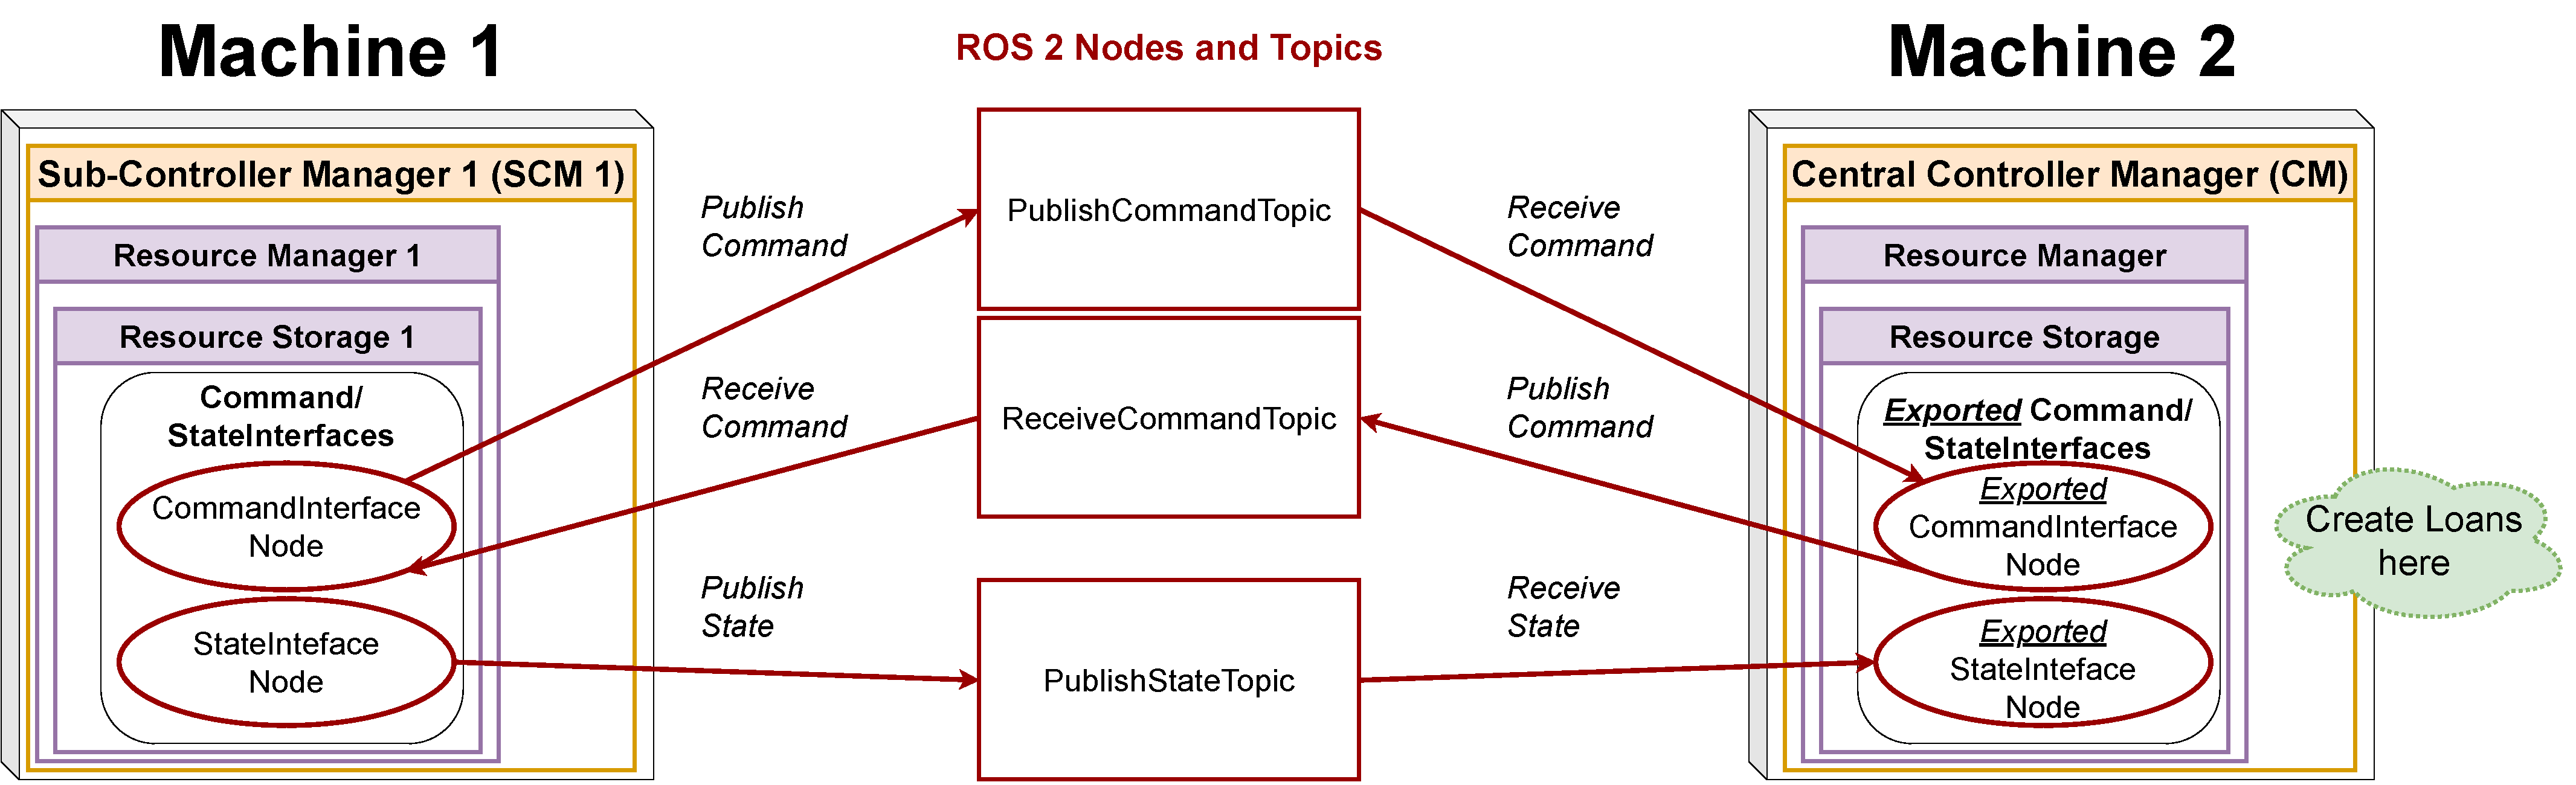
\includegraphics[width=1\textwidth]{Figures/C4/simple_concept.drawio.pdf}
	\caption{Schematic overview of the concept implemented.}
	\label{c4_fig_simple_concept}
\end{figure}
The fundamental idea of the design is to split the system at this point. 




\section{Integration in \gls{r2c}}

\subsection{Central Controller Manager}
\begin{itemize}
    \item \textbf{Subcontroller manager:}
    \begin{itemize}
        \item register subcontroller manager $\implies$ export descriptions of Command-/SystemInterfaces
        \item create publisher for Command-/StateInterfaces
        \item wait for registration to successfully complete
        \item subscribe to commandpublisher received from central controller manager
    \end{itemize}
    \item \textbf{Central Controller manager:}
    \begin{itemize}
        \item create service for registration
        \item register subcontroller manger if receive call
        \item subscribe to publisher of Command-/StateInteface of subcontrolelr manager
        \item create special Command-/StateInterfaces for this
        \item create publisher for Commands
        \item proceed as normal
    \end{itemize}
\end{itemize}
\begin{figure}[htbp]
	\centering
	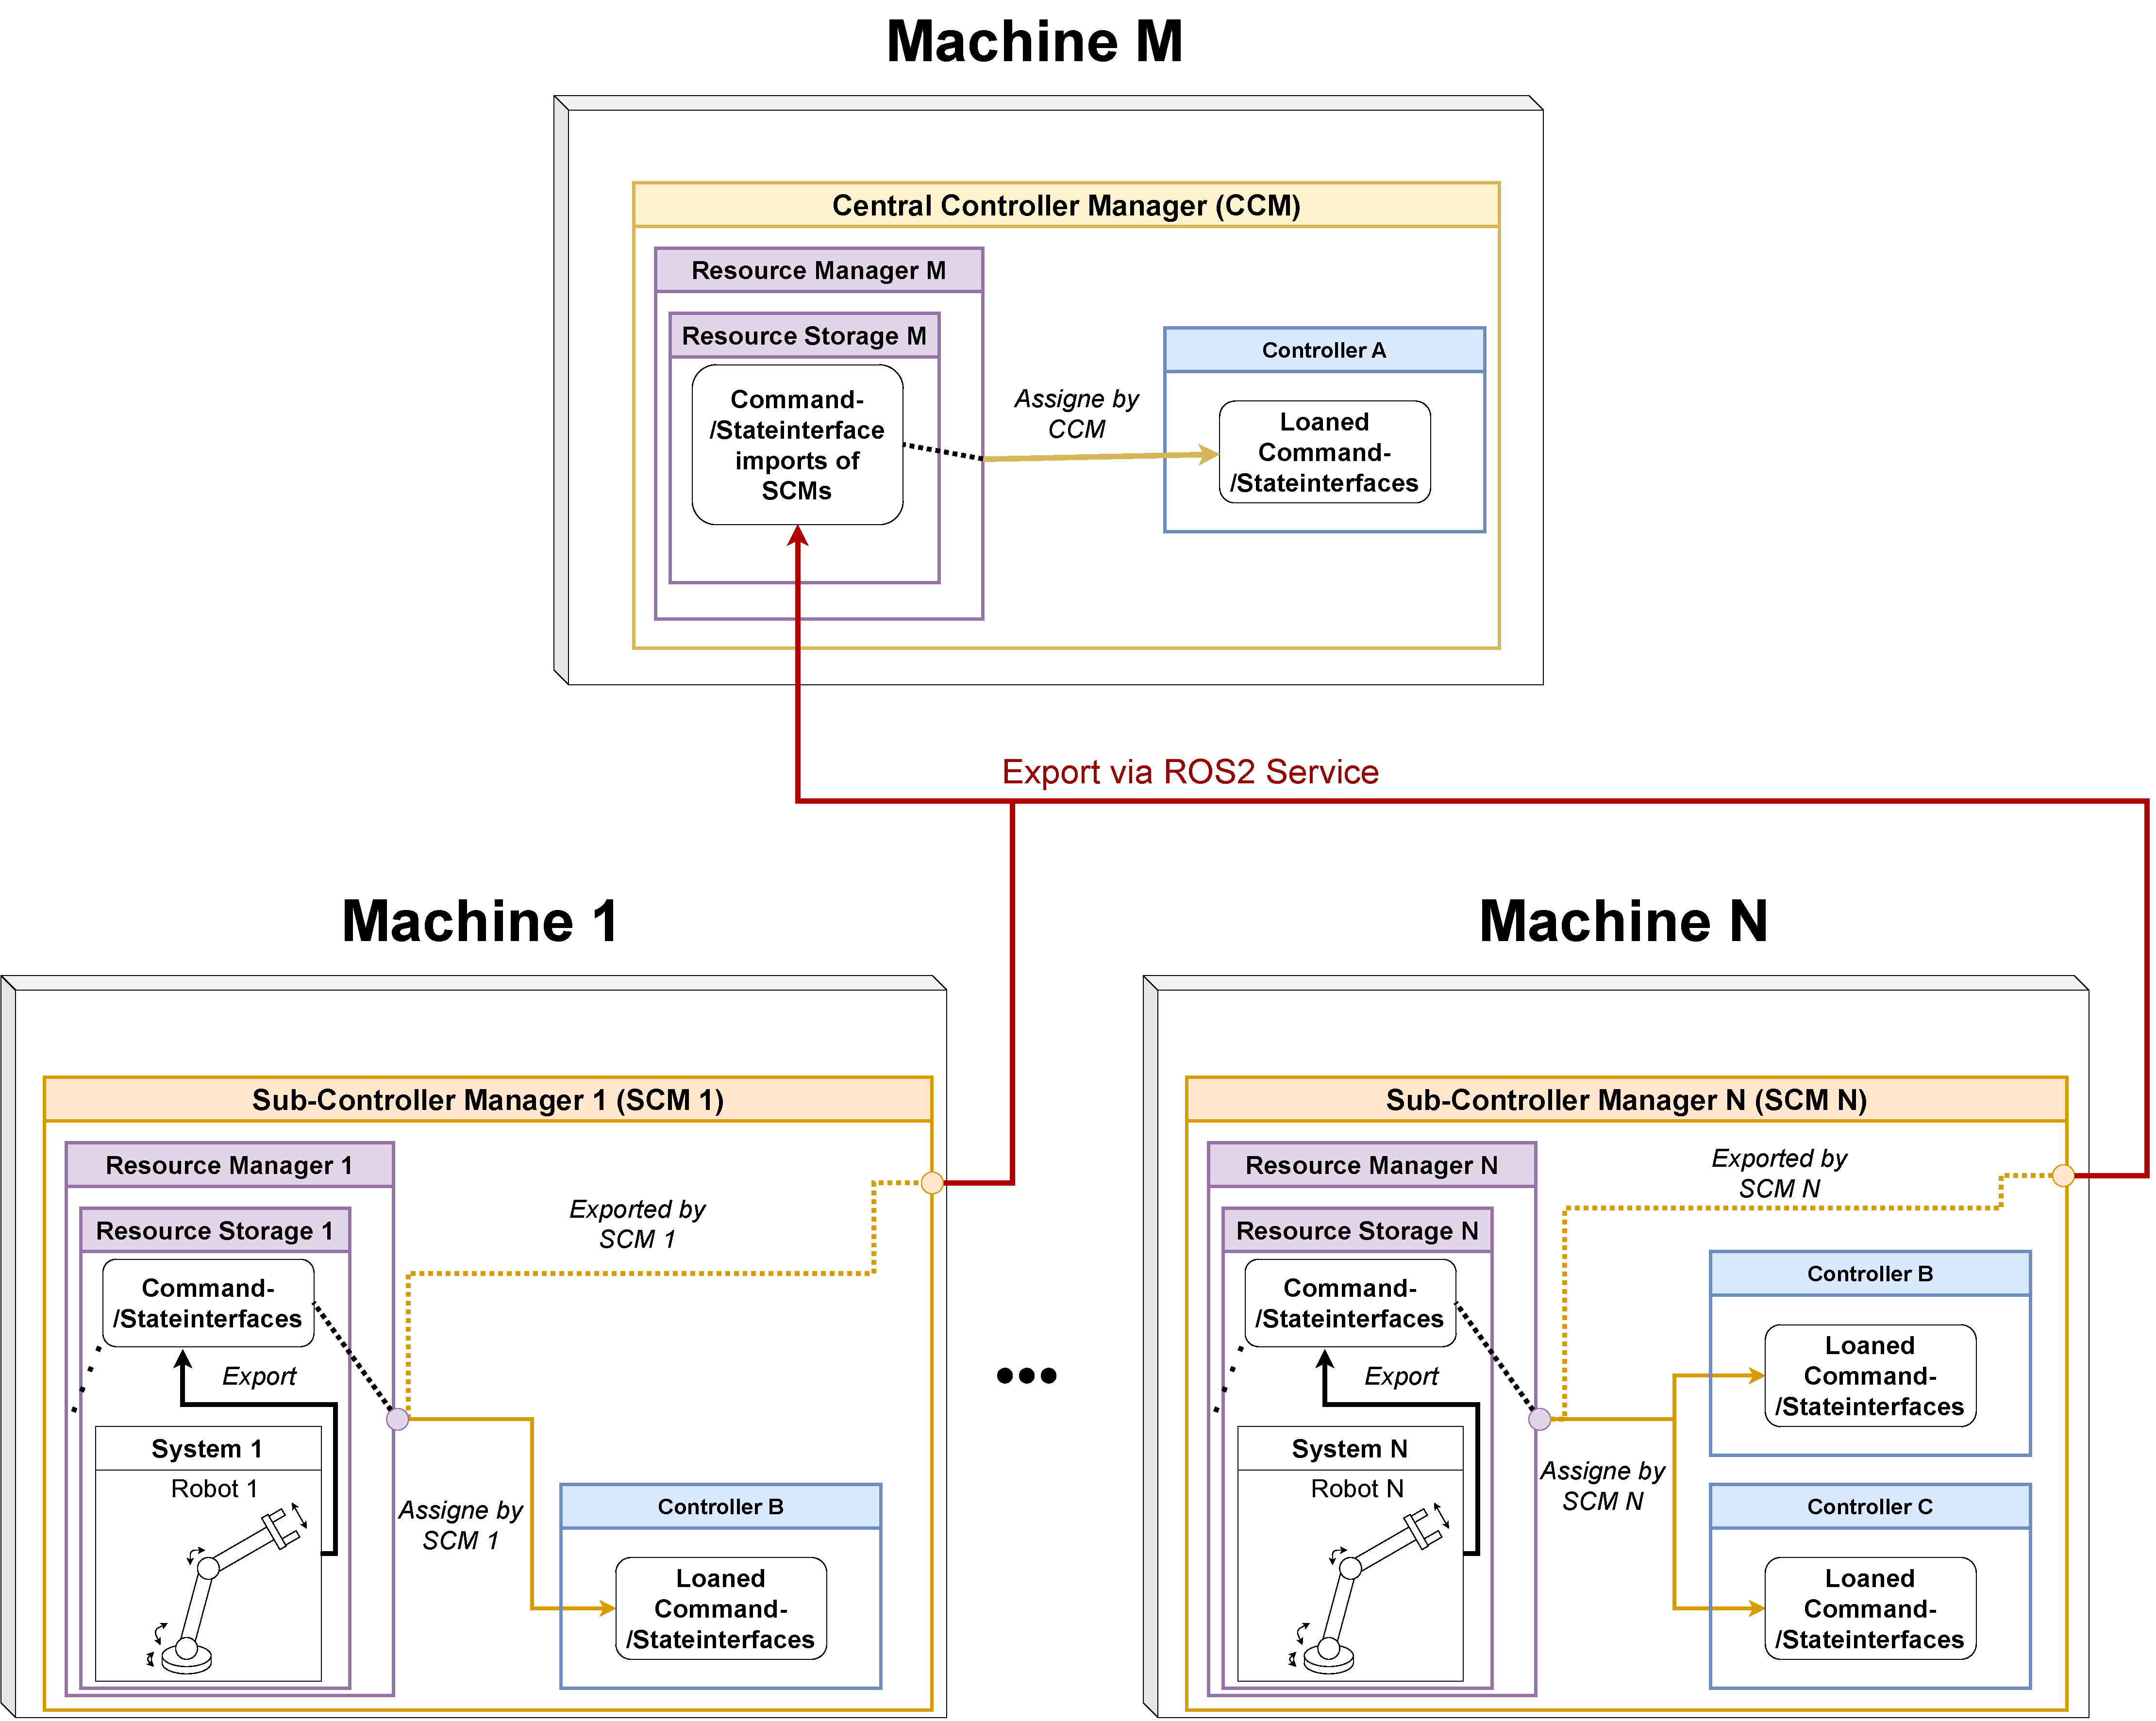
\includegraphics[width=1\textwidth]{Figures/C4/distributed_control.drawio.pdf}
	\caption{Schematic overview of the concept implemented.}
	\label{c4_fig_concept_overview}
\end{figure}

\subsection{Controller Chaining}
\begin{itemize}
    \item \textbf{Subcontroller manager:}
    \begin{itemize}
        \item same as for simple case
        \item export additionally reference interfaces
    \end{itemize}
    \item \textbf{Central Controller manager:}
    \begin{itemize}
        \item same as simple case
        \item import reference interfaces
        \item create chained controller
        \item proceed as normal
    \end{itemize}
\end{itemize}